\documentclass[conference]{IEEEtran}
\ifCLASSOPTIONcompsoc
  \usepackage[nocompress]{cite}
\else
  \usepackage{cite}
\fi
\ifCLASSINFOpdf
\else
\fi
\usepackage{multirow}
\usepackage{graphicx}
\usepackage{svg}
\begin{document}
\title{Stock Market Prediction using \\Artificial Intelligence}
\author{\IEEEauthorblockN{Rafael Isaac Cano Guitton}
\IEEEauthorblockA{School of Computer Science\\
Universidad Católica San Pablo \\
Arequipa, Perú \\
Email: rafael.cano@ucsp.edu.pe}
}
\maketitle
\begin{abstract}
Stock market has a nonlinear nature, research regarding forecasting and prediction model is one of the most important issues in recent years. 
People invest in stocks as if they were gambling and psychological factors can be several influential factors. This obviously makes it unprofitable 
and very unappealing for some individuals. Employing traditional analysis methods and strategies may also not ensure prediction reliability. In this 
paper we survey of current AI models approach to this task, how they are used, their datasets, performance and results. There also being room 
for improvement in future work by employing newer techniques and also testing models with dimension reduction.
\\\\
\textbf{Keywords: Stock  Market,  Deep Learning, Machine Learning , Prediction, Forecasting}
\end{abstract}
\IEEEpeerreviewmaketitle
\section{Introduction}
The stock market is a collection of markets where stocks of a firm are traded (bought and sold)\cite{M2018}.
Its behaviour is considered chaotic \cite{Singh2016} and it has consistently been vague for financial backers
due to the fact of several influential factors. This unreliable behaviour make investors live the potential to lose big sums of money, or to treat
the stock market as gambling. There is a correlation between investment psychology and market behaviour. With a predictive model, we can give a 
solution for impulsive market selling and buying. Assuring a percentage of reliability in trading this impulsive action can be reduced. While there is many automated ways to assist investors' decisions
in a timely manner\cite{nabipour2020predicting}, it is not enough to adress this first issue.
\\\\
The fundamental incentive behind forecasting is purchasing stocks that are probably going to increment in cost, and afterward selling stocks that are most likely going to fall\cite{nabipour2020predicting}. 
Stock costs respond to occasions identified with business execution or abroad business sectors. Financial backers judge based on specialized investigation, like organizations' diagrams\cite{Akita2016}.
\\\\
Now it is difficult to predict market trends and many AI approaches
have been investigated to predict them automatically. For example, investment simulation analysis with artificial
 markets\cite{Akita2016}.
\\\\
We will focus on Machine Learning and Deep Learning:
\\\\
\begin{itemize}
  \item Machine Learning: An AI field, probably the most known, that parses data, handles this data more efficiently and learns from that data. The main advantage is that, once
  the learning process is in a mature state, it can make informed decisions \cite{dey2016machine}. We use it in stock market prediction by learning patterns among big amounts of information.
  They can handle price fluctuations predictions to further develop trading techniques \cite{nabipour2020predicting}.
  \\\\
  \item Deep Learning: It is a subfield of AI, technically we can say that Deep Learning is Machine Learning.
  It is anything but a development of AI, it structures algorithms in layers to make an ANN (Artificial Neural Network), this enables accurate decisions
  without help from humans. The stock instability and nonlinearity present on the market cause problems for data analysts to develop a predictive model \cite{nabipour2020predicting}. And thus we can use Neural Networks for a predictive model.
\end{itemize}
Artificial Neural Networks are specially useful since its main usage is to recognize patterns. They are essentially simplified models of brains. In a brain, you have neurons, which are either activate or inactive,
and synapses, which connect the neurons together. The neurons are represented as simple booleans, and the synapses are represented by generally small numbers between negative one and one. The "weigth" of all the
synapses connected to a neuron determine its state \cite{M2018}.
\\\\
Training a Neural Network generally takes a lot of time, but using one to make predictions is very fast.
\\\\
For our datasets we can use news articles, financial reports and posts from microblogs made by analysts \cite{Vargas2017}. Using Recurrent Neural Networks(RNN) and Convolutional Neural Networks(CNN) we can
catch semantics from text and context information. We can also use data from individual stocks, gather data from each stock like: low, high, stock symbol, closing, average price, date and previous closing\cite{M2018}.
\\\\
The ample research literature, combined with the vast underlying models, tasks and training methods make it very
hard to identify the most appropriate approach or the most effective \cite{raghu2020survey}.
\\\\
And that is where our challenge resides. On this survey we aim to compare these techniques. We will compare prediction values for certain stocks with real stock market behavior. Also we will compare score based predictions for some approaches.
The purpose is to analyze current state of the art techniques for stock market accuracy\cite{Singh2016}.
% %\hfill mds
% %\hfill August 26, 2015
% %\subsection{Subsection Heading Here}
% %Subsection text here.
% %\subsubsection{Subsubsection Heading Here}
% Subsubsection text here.
% \section{Conclusion}
% The conclusion goes here.
\section{Related work}
ANN have been used in past decade in stock market prediction \cite{M2018}. ANN and HMM were proposed with the purpose to transform daily
stock values to independent group of prices as inputs to HMM \cite{nabipour2020predicting}. A common factor among current proposed models is that
an improvement to conventional neural networks is attempted. In Amir's study, nine ML methods (Adaboost, XGBoost,Random Forest,Decision Tree, NaïveBayes, SVC, KNN, ANN and Logistic Regression)
and two DL methods  (LSTM and RNN) were researched \cite{nabipour2020predicting} , putting special focus on performance.
They calculated indicators by stock exchaning values, using them as continuous data, and afterward changing indicators over to binary data prior to utilizing it. 
\\\\
In Amrita's study they used National Stock Exchange of India (NSE) and New York Stock Exchange (NYSE). Extracting day-wise closing price of stocks within different criteria, and then normaliznig data before feeding them to the
networks to train. They found similarities in patterns within those markets.
\\\\
There's also the textual information approach, in Vargas' proposal \cite{Vargas2017} they used 106.494 news articles
from Reuter's website, aiming to the topic of financial news. They found that using titles is more useful than the entire article for forecasting purposes,
so their proposed model only uses news titles. Now the proposed model uses only news from the day before the forecasting day, comparing them to models that use news from past day, week and month,
Vargas' model outperforms said models. On textual information approaches, Akita's proposal \cite{Akita2016} also uses financial news, but they also use numerical information. They use them to predict 10 companies' closing stock prices by regression.
Also learning correlation between companies. This since news from a company can have an effect in several companies' stock pricing within the same industry. 

\section{Predictive Models}
Taking in account research mentioned in related work, algorithms used for stock market prediction were clasified. This so we can have an overview of which techniques were used
and how these were applied. If there was preprocessing of data so we can know if that can have an impact.
\\\\
A classification based on dataset type was also made, this since several techniques were used in both cases but having  different results. 
\\\\
Therefore we will have our models classified by:
\begin{itemize}
  \item Machine Learning Algorithms.
  \item Deep Learning Algorithms.
\end{itemize}
Also describing preprocessing and dataset type.
\begin{table}[]
  \caption{Models by Technique}
\begin{center}
  \begin{tabular}{|p{1.5cm}|p{2.1cm}|p{2.2cm}|p{1.5cm}|}
    \hline
    Technique                         & Models                                                & Preprocessing                                                 & Dataset type                                               \\ \hline
    Deep Learning    & CNN \cite{M2018} \cite{Vargas2017}                                                  & Data Normalization                                            & \multicolumn{1}{c|}{\multirow{2}{*}{Textual \& Numerical}} \\ \cline{2-3}
                                      & RNN\cite{M2018}\cite{Singh2016}\cite{Vargas2017}                                               & Data Normalization \& Converting continuous data (indicators) & \multicolumn{1}{c|}{}                                      \\ \cline{2-4} 
                                      & (2D)²PCA + DNN \cite{Singh2016}                                       & -                                                             & \multirow{11}{*}{Numerical}                                \\ \cline{2-3}
                                      & (2D)²PCA + RBFNN \cite{Singh2016}                                     & -                                                             &                                                            \\ \cline{2-3}
                                      & DNN \cite{nabipour2020predicting}                     & -                                                             &                                                            \\ \cline{2-3}
                                      & MLP \cite{M2018}                                                  & Data Normalization                                            &                                                            \\ \cline{2-3}
                                      & LSTM \cite{M2018} \cite{Akita2016}                                                 & Data Normalization \& Converting continuous data (indicators) &                                                            \\ \cline{2-3}
                                      & ANN \cite{nabipour2020predicting} \cite{deepak2017machine}                                                 & -                                                             &                                                            \\ \cline{1-3}
    Machine Learning & KNN \cite{nabipour2020predicting}                                                 & Converting continuous data (indicators)      &                                                            \\ \cline{2-2}
                                      & Adaboost \cite{nabipour2020predicting}                                             &                                                               &                                                            \\ \cline{2-2}
                                      & XGBoost \cite{nabipour2020predicting}                                              &                                                               &                                                            \\ \cline{2-2}
                                      & SVC \cite{nabipour2020predicting}                                                  &                                                               &                                                            \\ \cline{2-2}
                                      & \begin{tabular}[c]{@{}c@{}}Naïve\\ Bayes\end{tabular} \cite{nabipour2020predicting} \cite{reddy2018stock} &                                                               &                                                            \\ \hline
    \end{tabular}
  \label{tab:comp}
  \end{center}
  \end{table}

\begin{figure*}[htbp]
  \centerline{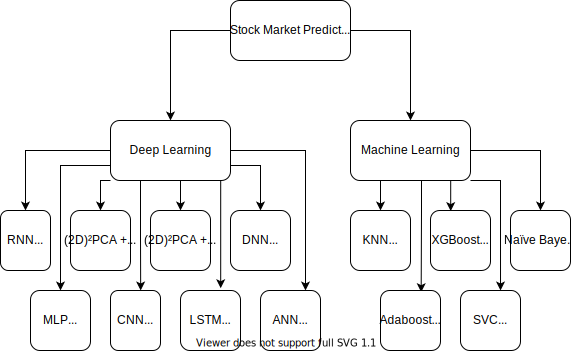
\includegraphics[scale=.60]{mapita.png}}
  \caption{Paper classification}
  \label{fig}
\end{figure*}

\subsection{Machine Learning Algorithms}
In Nabipour's approach \cite{nabipour2020predicting}, in order to use machine learning models, their steps were:  normalizing features for their continous data, randomly splitting the main dataset into train data
and test data, fitting the models and evaluating them by validation data to prevent overfitting, and using metrics for final evaluation with test data.
A brief listing of Machine Learning Algorithms that were reviewed:
\subsubsection{K-Nearest Neighbors}
A method non-parametric for classification and regression, it is supervised and based on instances. It does not learn from a model explicitly, it memorizes
the instances of training that are used as a "knowledge base" for prediction phase.
\\\\
Now to apply KNN we have two properties suggested, non-parametric algorithm and lazy learning, this in light of the fact that there is not any supposition for underlying data distribution.
On Nabipour's approach \cite{nabipour2020predicting}, they used 100 Neighbors and K-dimensional tree algorithm for their KNN prediction approach.
\\\\
\subsubsection{Adaptative Boosting}
It is a boosting technique that is used as an Ensemble Method. Its purpose is to train weak learners sequentially in order to adjust their past predictions. It can be defined as a 
meta-predictor that begins by fitting a model on the basic dataset prior to fitting additional copies of it on the same dataset. During train cycle, samples' weights are adjusted based on the current 
prediction error error; consequently, the subsequent model focuses on tough items \cite{nabipour2020predicting}.
\\\\
On Nabipour's approach \cite{nabipour2020predicting}, the parameters for their Adaboost were: a Max Depth of, for their estimator they used a decision tree, having from 50 to 500 trees progressing in a rate of 50, and a learning rate of 0.1.
\\\\
\subsubsection{eXtreme Gradient Boosting}
It provides an efficient and effective implementation of the gradient boosting algorithm, designed to be computionally efficient
and highly effective. Similarly to Adaboost, it utilizes the principles of Boosting for weak learners but , compared to other tree-based models, it achieves superior speed and performance. It has the advantages of regularization in order to avoid
overfitting, proficient handling of missing data, catch awareness, in-built cross-validation capabilities, paralelized tree building and pruning.
\\\\
On Nabipour's approach \cite{nabipour2020predicting}, the parameters for their XGBoost were: a Max Depth of 10, having from 50 to 500 trees progressing in a rate of 50, and Logistic Regression for Binary classification as their objective.
\\\\
\subsubsection{Support Vector Clasifier}
Supervised learning model, its objective is to find a hyperplane in an N-dimensional space that
precisely classifies the data points. Its purpose is to maximize the margin between the hyperplane and data points.
\\\\
For SVC, on Nabipour's approach \cite{nabipour2020predicting}, they used Linear, Poly(degree=3),RBF, Sigmoid for Kernel, a C of 1.0 and their Gamma value was 1/((num)x(variance)) f:features.
\\\\
\subsubsection{Naïve Bayes}
It is a probabilistic method that is based in Bayes' theorem, called Naive since given some additional simplifications that determine
the independance hipotesis of predict variables.
\\\\
For Naïve Bayes, on Nabipour's approach \cite{nabipour2020predicting}, they used Gaussian Algorithm, for their Gamma value they used 1/((num)x(variance)) f:features, and a C value of 1.0.
\\\\
There were several classification metrics across papers to evaluate performance of models,
among of which we can metion F1-Score, accuracy, receiver operating characteristics \cite{nabipour2020predicting},
Mape (Mean Absolute Percentage Error) \cite{M2018}, effectivenes of Paragraph Vector, effectivenes of LSTM \cite{Akita2016}, index prediction \cite{Vargas2017},
forecast values, Total Return (TR), Hit Rate (HR) and Root Mean Square Error (RMSE) \cite{Singh2016}.
\\\\
According to Deepak \cite{deepak2017machine}, Naïve Bayes by itself can and is used for automatic stock purchase model. In the real world it is used to develop web portals for automatic trading.
\\\\
Each of the machine learning models have their limitations when it comes to solve the stock market prediction problem.
For training machine learning models in Nabipour's approach \cite{nabipour2020predicting}, they normalized features, randomly split 
the main dataset into train data and test data, fitting the models and evaluating them by validation data. When an extra layer to convert continuous data to binary
one based on the nature and property of the features there was a clear improvement. So continuous data has terrible performance on every model except some Deep Learning ones, so they are unviable with machine learning. Binary data on the other hand holds the aformentioned
improvement to the level of up to 83 percent. This since the layer that converts to it is able to convert non-stationary values to trend deterministic ones.
\\\\
Now despite it is clear performance disadvantage towards deep learning models, machine learning models have a better runtime performance. This due to the fact
that less computational power is required for prediction. This combined with binary data on Nabipour's approach \cite{nabipour2020predicting}, gets no less than 0.83 F1 score which would make it
a viable option. This being metioned, some are already used as mentioned on Deepak's paper \cite{deepak2017machine}, you can make algorithmic trading bots but it is limited to favourable outcome and will not provide stock analysis.



\subsection{Deep Learning Algorithms}

On Nabipour's approach \cite{nabipour2020predicting}, they used values that were three-dimensional (features, time-steps, samples ), so they reshaped the input values by utilizing a function. A dropout layer and weight regularization are utilized as well for overfitting prevention.
A brief listing of Deep Learning Algorithms that were reviewed:

\subsubsection{Convolutional Neural Network}
It is an ANN (Artificial Neural Network) which uses supervised learning. It processes layers emulating the how in the human eye the visual cortex works to identify several characteristics on entries that definetly allow it to classify (through identification) objects, these based in patterns.
\\\\
On Hiransha's approach \cite{M2018}, their CNN almost captured the pattern between 1500 and 2300 days considering that for a particular window only the data in it is accounted for. Within a different stock it actually failed to capture variation in system at intervals of 1400 and 1800 days.
\\\\
\subsubsection{Recurrent Neural Network}
A kind of neural networks, that as its name suggets allows past outputs to be utilized as inputs whilst having hidden strates. RNNs are able to process inputs of any length and take them from two sources one being from the present
and the other one from the past. Afterward, information from the aformentioned sources are utilized on making the decision of how they react to the new set of data.
\\\\
On Hiransha's approach \cite{M2018} their RNN failed to recognize the seasonal pattern which can be considered as change in behaviour of system. On a different stock, success was almost achieved by it at recognizing the pattern.
\\\\
With Nabipour's approach \cite{nabipour2020predicting} since RNN has a recurrent nature, they had the model be fed with input data taken from a range of one to 30 days' technical indicators. Their parameters were 500 Hidden Layer Neuron Count, 1-2-5-10-20-30 for number of training days, both Tanh and softmax as activation function, learning rate of 0.00005, $B_1$ of 0.9, $B_2$ of 0.999 for optimizer, Max EPOCHS OF 10000 and their training stop condition
was: Early stopping: monitoring parameter = validation data accuracy patience = 100 epochs. 
\\\\
\begin{figure*}[htbp]
  \centerline{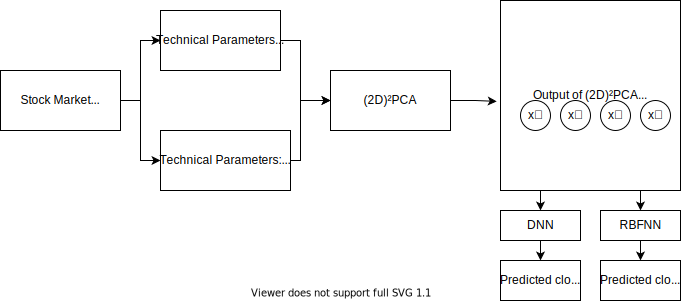
\includegraphics[scale=.65]{mapita2.png}}
  \caption{2-Directional 2-Dimensional Principal Component Analysis}
  \label{fig}
\end{figure*}
\subsubsection{2-Directional 2-Dimensional Principal Component Analysis + Radial Basis Function Neural Network}
The main idea behind (2D$)^2$PCA is that it is based on 2D matrices as opposed to the standar PCA, it has higher accuracy. It is used for dimensionality reduction in
the researched proposals. Its output is fed to the RNN.
\\\\
Since the main idea behind this approach is to use dimension reduction to the dataset, it projects our original raw data matrix into a projection matrix and information loss ocurrs,
but the obvious advantage is that the time to process is lower and the model's convergence speed increments many overlay.
\\\\
With Singh's approach\cite{Singh2016}, it was found that compared to RNN (that was performing poorly) there is a 15.6\% improve. 
\\\\
\subsubsection{2-Directional 2-Dimensional Principal Component Analysis + Deep Neural Network}
Same as last but its output is instead fed to Dimension Neural Network, which is the most simple neural network, it has some level of complexity, usually two layers. Now, the dimensional reduction provided by 
(2$D)^2$)PCA is recommended for large datasets, since the aformentioned information loss wouldn't cause variation in the output.
\\\\
Compared to RBFN with (2$D)^2$)PCA on Sing's approach\cite{Singh2016}, the existing method they used for comparison had a worse performance than their proposal. Results demonstrated that their model provided an accuracy improvement of 4.8\% in regards to hit rate for a window size value of 20. So compared to RNN and (2D)²PCA+RBFNN, it is proved to be the better predictor in regards of trend prediction within stock market.
\\\\
\subsubsection{Multilayer Perceptron}
Also known as feed forward neural network, a simple sample of a neural network. Through a weighted matrix,individual input neurons get linked to the succeeding hidden layer.
\\\\
On Hiransha's approach \cite{M2018}, MLP had a mixed performance, having identified the pattern in the beginning for AXIS BANK stock in the 1400 to 1700 days period. But was overall the most successful model since it captured the seasonal pattern for HCLTECH between 1600 and 1900 days.
\\\\
\subsubsection{Long Short-Term Memory}
A kind of RNN capable of leaning order dependence in sequence prediction problems. A behaviour specially usefull to process our datasets. 
\\\\
On Akita's approach \cite{Akita2016}, a LSTM was trained for 50 epochs with Adam, with one layer and were unrolled 20 steps, they also applied 50 percent dropout on the non recurrent connections.
Now comparing it to an MLP it achieved higher profits in all industries, also achieving higher profits in 4 out of 5 industries comparing it to SVR. In their comparison, LSTM significantly outperformed simple-RNN.
On Nabipour's approach \cite{nabipour2020predicting} since LSTM has a recurrent nature, they considered and rearranged technical indicators of a range within one to thirty days, this to be fed into the model. Their parameters were 500 Hidden Layer Neuron Count, 1-2-5-10-20-30 for number of training days, both Tanh and softmax as activation function, learning rate of 0.00005, $B_1$ of 0.9, $B_2$ of 0.999 for optimizer, Max EPOCHS OF 10000 and their training stop condition
was: Early stopping: monitoring parameter = validation data accuracy patience = 100 epochs.
On Hiransha's approach \cite{M2018} similarly to their RNN, their LSTM was not successful at  identify the seasonal pattern and also failed to capture change in system between 1400 and 1800 days.
\\\\
\subsubsection{Artificial Neural Network}
Usually single or multilayer nets whuch fully are fully connected together. It is able to form the network deeper due to the number of hidden layers being rised.
\\\\
On Nabipour's approach \cite{nabipour2020predicting} the parameters they used for their ANN were: Hidden Layer Neuron Count of 20,50,100,200,500; ReLU, Sigmoid, Tanh as activation functions; $B_1$ of 0.9, $B_2$ of 0.999 for optimizer; and their training stop condition
was: Early stopping: monitoring parameter = validation data accuracy patience = 100 epochs.
\\\\
Since Deep Learning models are more robust on predicting tasks, their performance is always better than Machine Learning models.
On Akita's approach \cite{Akita2016}, they use Paragraph Vector in order to achieve the distributed representation by getting variable length pieces of text mapped to a fixed-length vector.
Now they use to categories where them to get classified into, these being Distributed Bag of Words version of Paragraph Vector(PV-DBOW) and Distributed Memory of Paragraph Vectors(PV-DM). For their expermients they used a combination of Numerical and Textual
information, but they also compared it with only numerical information. In four out of five indistries higher profits were achieved by it, also the total happened to be by 490 points higher as well. So it was effective to employ distributed representations
by using their aformentioned Paragraph Vector. They simulated real-world stock trading effectively doing Market Simulation. LSTM and RNN were tested on this artificial market and despite both being able of acknowledging time series data, LSTM
significantly outperformed Simple-RNN, this since LSTM has nondeterministic transactions. This meaning LSTM was capable of capturing robustly fluctuating time series changes.
When using binary data on Nabipour's approach \cite{nabipour2020predicting}, although there were only 2 deep learning models used (RNN and LSTM), they showed a clear superiority for the predictive task, this time having RNN be superior to LSTM but with a smaller margin.
In Textual Information exclusively for Manuel's approach \cite{Vargas2017}, they made heavy comparisons between CNN and RNN based models. Using a classification of inputs from the dataset being word embedding input, sentence embedding input, bag of word, structure events tuple input, sum of each word in a document and event embedding.
Their results show that, comparing word embedding and sentence embedding, the first one comes out as the superior. And that the RCNN proposed approach layering RNN and CNN compared to only CNN is better on index prediction architecture-wise. This proposed model outperforms all baseline models with the expection of EB-CNN, this is likely ue to event embedding that is a more powerful method
to model the concent in news articles. This also shows that a very important factor to be considered when construction a prediction model is architecture.


\section{Conclusion and future work}
\subsubsection*{Conclusion}
This paper analyzed and compared various prediction models across several research papers. Making focus in prediction that was we know, has a key role in trading that on its own is very complex and challenging process \cite{sharma2017survey}. Considering Deep Learning applied to Natural Language Processing and Image Recognition task as a success, its pretty tempting to apply AI to Stock Market Prediction. Researched methods showed that not only is it possible to predict certain trends but that there exist some models that are
currently used in real life for assissted trading and automatic trading. Short term forecasting or day trading is also more accurate in some work.
\\
Nevertheless it was also proven that it has not, and probably will not reach the point where it can accurately predict the future of (any) market consistently
There is many ways to implement a model, going from using numerical, textual or both as datasets. These models can be trained to create its own trading strategy.
\\\\
As mentioned, input data plays an important role in prediction, and with use of Numerical data we get high performance and efficiency on Machine Learning models. So performance also plays a core role in Stock Market Prediction model at least in forecasting for day-trading. We could define and implement a model. Resources, strategy and market will
also have an impact on how effective models can be. How this data is treated is also important since converting continuous data to binary data also proved effective in performance gains.
\\\\
To sum it all up, there is promising methods for this task and some of the approaches could be applied to real life trading strategies, some on the analysis side and some could just perform their own operations with their strategies. Both Machine Learning and Deep Learning models are effective, it will just depend on how you expect to use the model.
\subsubsection*{Future work}
As research continues and new algorithms arise like Deep Belief Network, Regularization, Autoencoders and Advanced Optimization, a comparison needs to be made.
\\
Regarding dimension reduction, there is not enough work testing this technique and it would be interesting since it was shown that it can improve performance. Specially since Stock Market Prediction datasets tend to be large.
\bibliographystyle{IEEEtran}
\bibliography{references}
\end{document}